%%%%%%%%%%%%%%%%%%%%%%%%%%%%%%%%%%%%%%%%%
% Beamer Presentation
% LaTeX Template
% Version 1.0 (10/11/12)
%
% This template has been downloaded from:
% http://www.LaTeXTemplates.com
%
% License:
% CC BY-NC-SA 3.0 (http://creativecommons.org/licenses/by-nc-sa/3.0/)
%
%%%%%%%%%%%%%%%%%%%%%%%%%%%%%%%%%%%%%%%%%

%----------------------------------------------------------------------------------------
%   PACKAGES AND THEMES
%----------------------------------------------------------------------------------------

\documentclass{beamer}

\mode<presentation> {}

% The Beamer class comes with a number of default slide themes
% which change the colors and layouts of slides. Below this is a list
% of all the themes, uncomment each in turn to see what they look like.

\usetheme{default}
%\usetheme{AnnArbor}
%\usetheme{Antibes}
%\usetheme{Bergen}
%\usetheme{Berkeley}
%\usetheme{Berlin}
%\usetheme{Boadilla}
%\usetheme{CambridgeUS}
%\usetheme{Copenhagen}
%\usetheme{Darmstadt}
%\usetheme{Dresden}
%\usetheme{Frankfurt}
%\usetheme{Goettingen}
%\usetheme{Hannover}
%\usetheme{Ilmenau}
%\usetheme{JuanLesPins}
%\usetheme{Luebeck}
%\usetheme{Madrid}
%\usetheme{Malmoe}
%\usetheme{Marburg}
%\usetheme{Montpellier}
%\usetheme{PaloAlto}
%\usetheme{Pittsburgh}
%\usetheme{Rochester}
%\usetheme{Singapore}
%\usetheme{Szeged}
%\usetheme{Warsaw}

% As well as themes, the Beamer class has a number of color themes
% for any slide theme. Uncomment each of these in turn to see how it
% changes the colors of your current slide theme.

%\usecolortheme{albatross}
%\usecolortheme{beaver}
%\usecolortheme{beetle}
%\usecolortheme{crane}
%\usecolortheme{dolphin}
%\usecolortheme{dove}
%\usecolortheme{fly}
%\usecolortheme{lily}
%\usecolortheme{orchid}
%\usecolortheme{rose}
%\usecolortheme{seagull}
%\usecolortheme{seahorse}
%\usecolortheme{whale}
%\usecolortheme{wolverine}

%\setbeamertemplate{footline} % To remove the footer line in all slides uncomment this line
%\setbeamertemplate{footline}[page number] % To replace the footer line in all slides with a simple slide count uncomment this line

%\setbeamertemplate{navigation symbols}{} % To remove the navigation symbols from the bottom of all slides uncomment this line


\usepackage{graphicx} % Allows including images
\usepackage{booktabs} % Allows the use of \toprule, \midrule and \bottomrule in tables
\usepackage{xcolor}   % Allows for change of font color
\usepackage{algorithm}
\usepackage{mathtools}
\usepackage{algpseudocode}
\usepackage{bm}
\usepackage{calc}
\usepackage{etoolbox}
\usepackage{array}
\usepackage{amssymb}% http://ctan.org/pkg/amssymb
\usepackage{pifont}% http://ctan.org/pkg/pifont
\setbeamertemplate{mini frames}{}

%----------------------------------------------------------------------------------------
%   TITLE PAGE
%----------------------------------------------------------------------------------------

%\AtBeginSection[]
%{
%  \begin{frame}<beamer>
%    \frametitle{Outline for Section \thesection}
%    \tableofcontents[currentsection]
%  \end{frame}
%}

\setbeamertemplate{theorems}[numbered]
\pretocmd{\part}{\setcounter{theorem}{0}}{}{}
\newtheorem{proposition}[theorem]{Proposition}

\newcommand{\cmark}{\ding{51}}%
\newcommand{\xmark}{\ding{55}}%

\begin{document}

\section[Application]{Appplication of QAP in Modulation Diversity (MoDiv)
Design}

\subsection[Backgrounds]{Backgrounds}

\begin{frame}
  \frametitle{Modulation Mapping}
    \begin{columns}[c]
      \column{.12\textwidth}
        \begin{tabular}{c|c}
          \hline
          $p$ & bits \\
          \hline
          0 & 0000 \\
          \alert<2>{1} & \alert<2>{0001} \\
          2 & 0010 \\
          \ldots & \ldots \\
          15 & 1111 \\
          \hline
        \end{tabular}
        
      \column{.03\textwidth}
      $\xrightarrow{\mbox{Map}}$
      
      \column{.2\textwidth}
      \includegraphics<1>[height=3cm]{./figs/16QAM_bare.pdf}
      \includegraphics<2>[height=3cm]{./figs/16QAM_bare_marked.pdf}
      
      \column{.07\textwidth}
      $\xrightarrow{\mbox{Channel}}$
      
      \column{.25\textwidth}
      \includegraphics<1>[height=3.5cm]{./figs/constellation_diagram.pdf}
      \includegraphics<2>[height=3.5cm]{./figs/constellation_diagram_marked.pdf}
      
    \end{columns}
    \begin{itemize}
      \item Unideal wireless channel tends to cause demodulation errors.
      \item Constellation points closer to each other are more likely to be
      confused.
    \end{itemize}
    Modulation mapping needs to be carefully designed!
\end{frame}

\begin{frame}
  \frametitle{Single Transmission: Gray-mapping}
    \begin{block}{Strategy (Gray-mapping)}
      Neighboring constellation points ({\color{red} horizontally} or
      {\color{blue} vertically}) differ only by 1 bit, so as to
      minimize the Bit Error Rate (BER).
    \end{block}
    \begin{figure}
      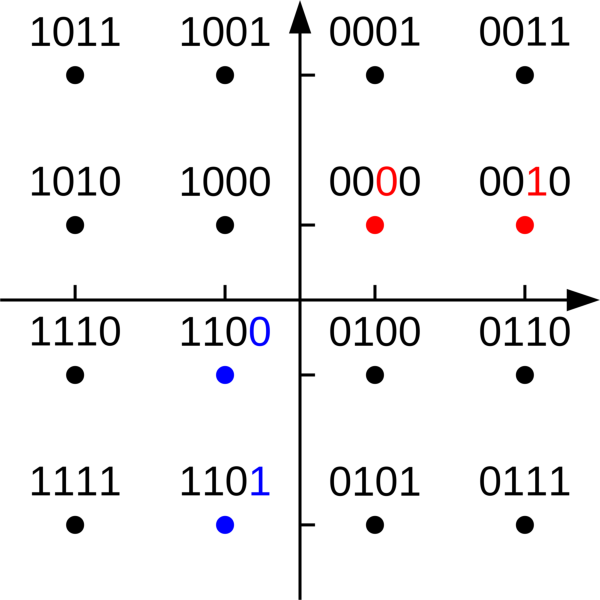
\includegraphics[width=0.4\textwidth]{figs/16QAM_Gray.pdf}
      \caption{Gray-mapping for 16-QAM, 3GPP TS 25.213.}
    \end{figure}
\end{frame}

\begin{frame}
  \frametitle{HARQ with Constellation Rearrangement (CoRe)}
  \begin{block}{Hybrid Automatic Repeat reQuest (HARQ)}
    \begin{itemize}
      \item Same piece of information is retransmitted again and again, and
      combined at the receiver until it is decoded successfully or expiration.
      \item An error control scheme widely used in modern wireless systems such
      as HSPA, WiMAX, LTE, etc.
    \end{itemize}
  \end{block}
  \begin{block}{Constellation Rearrangement (CoRe)}
    \begin{itemize}
      \item For each round of retransmission, different modulation mappings are
      used (explained next).
      \item Exploit the Modulation Diversity (MoDiv).
    \end{itemize}
  \end{block}
\end{frame}

\begin{frame}
  \frametitle{An Example of CoRe}
  \begin{columns}[c]
    \column{.5\textwidth}<1->
    \begin{figure}
      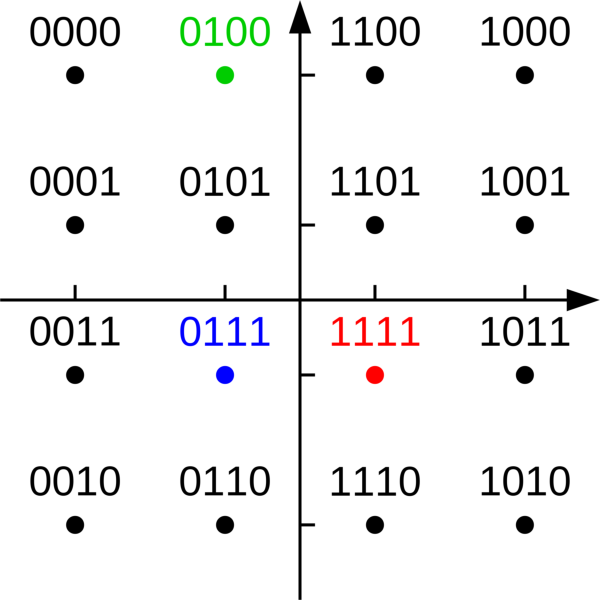
\includegraphics[width=0.6\textwidth]{figs/CoRe_0.pdf}
      \caption{Original transmission.}
    \end{figure}
    
    \column{.5\textwidth}<2>
    \begin{figure}
      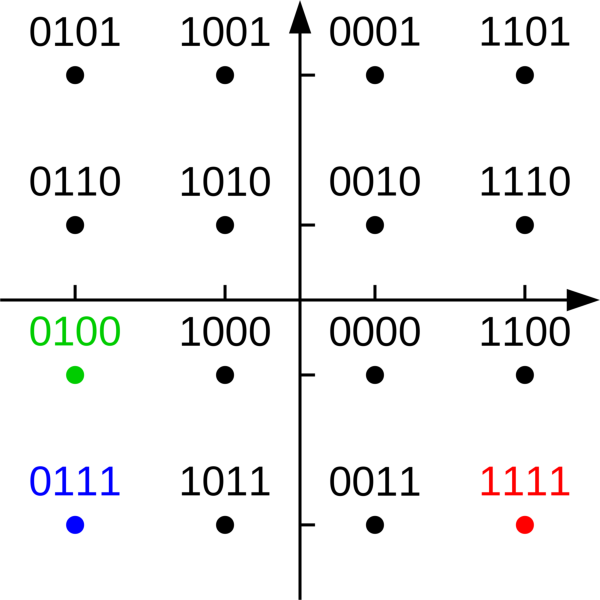
\includegraphics[width=0.6\textwidth]{figs/CoRe_1.pdf}
      \caption{First retransmission.}
    \end{figure}
  \end{columns}
  
  \begin{itemize}
    \item<1-> Original transmission: {\color{blue} 0111} is easily confused with
    {\color{red} 1111}, but well distinguished from {\color{green} 0100}.
    \item<2> First retransmission: {\color{blue} 0111} should now be mapped far away from {\color{red} 1111},
    but can be close to {\color{green} 0100}.
  \end{itemize}
\end{frame}

\begin{frame}
  \frametitle{General Design of MoDiv Through CoRe}
  \begin{block}{Challenges}
    \begin{enumerate}
      \item More than 1 retransmissions?
      \item More general wireless channel models?
      \item Larger constellations (e.g. 64-QAM)?
    \end{enumerate}
  \end{block}
  
  We formulated 2 different MoDiv design problems into \alert{Quadratic
  Assignment Problems (QAPs)} and demonstrate the performance gain over existing
  CoRe schemes.
\end{frame}

\subsection[MoDiv for TWRC-HARQ]{MoDiv Design for Two-Way Amplify-and-Forward
Relay HARQ Channel}
\begin{frame}
  \frametitle{Two-Way Relay Channel (TWRC) with Analog Network Coding (ANC)}
  \begin{itemize}
    \item<1-> System components: 2 sources ($S_1$, $S_2$) communicate with each
    other with the help of 1 relay ($R$).
    \item<2-> Alternating between 2 phases:
      \begin{itemize}
        \item<2-> Multiple-Access Channel (MAC) phase: the 2 sources transmit to
        the relay simultaneously.
        \item<3> Broadcast Channel (BC) phase: the relay amplify and broadcast
        the signal received during the MAC phase back to the 2 sources
      \end{itemize}
  \end{itemize}
  \vfill
  \begin{columns}[t]
    \column{.5\textwidth}
    \begin{figure}
      \includegraphics<1>[width=0.8\textwidth]{figs/model.pdf}
      \includegraphics<2>[width=0.8\textwidth]{figs/model_MAC.pdf}
      \includegraphics<3>[width=0.8\textwidth]{figs/model_BC.pdf}
      \caption{TWRC-ANC channel.}
    \end{figure}
    
    \column{.5\textwidth}
    \only<2>{
      \begin{align*}
        y_R = h_1x_1+h_2x_2+n_R
      \end{align*}
    }
    \only<3>{
      \begin{align*}
        y_1 &= \alpha g_1 y_R + n_1, \\
        y_2 &= \alpha g_2 y_R + n_2
      \end{align*}
    }
    
  \end{columns}
\end{frame}

\begin{frame}
  \frametitle{HARQ-Chase Combining (CC) Protocol}
  \begin{itemize}
    \item $Q$: size of the constellation.
    \item $M$: maximum number of retransmissions.
    \item $\psi_m[p]$, $m=0,\ldots, M$, $p=0,\ldots,Q-1$: constellation mapping
    function between ``label'' $p$ to a constellation point for the $m$-th
    retransission.
  \end{itemize}
  Due to symmetry of the channel, consider the transmission from $S_1$ to $S_2$
  only. The received signal during the $m$-th retransmission of label $p$ is:
  \only<1>{
    \begin{align*}
      y_2^{(m)} = \alpha^{(m)} g_2^{(m)}(h_1^{(m)}\psi_m[p] +
      {\color{red}h_2^{(\tilde{m})}\psi_{\tilde{m}}[\tilde{p}]} + n_R^{(m)}) +
      n_2^{(m)},
    \end{align*}
  }
  \only<2>{
    \begin{align*}
      y_2^{(m)} = \alpha^{(m)} g_2^{(m)}(h_1^{(m)}\psi_m[p] + n_R^{(m)}) +
      n_2^{(m)},\, \mbox{(after SIC)}
    \end{align*}
  }
\end{frame}

\begin{frame}
  \frametitle{HARQ-Chase Combining (CC) Protocol (Continued)}
  The receiver combines all the received symbols across all
  retransmissions so far until decoding is determined successful.
  \begin{center}
    \includegraphics<1>[height=3cm]{./figs/ml.pdf}
    \includegraphics<2>[height=3cm]{./figs/ml_1.pdf}
    \includegraphics<3>[height=3cm]{./figs/ml_m.pdf}
  \end{center}
  \begin{block}{Maximum Likelihood (ML) detector}
    \begin{align*}
      p^* = \arg\min_p\sum_{k=0}^{m} \frac{|y_2^{(k)} -
      \alpha^{(k)} g_2^{(k)} h_1^{(k)}\psi_k[p]|^2}
      {\sigma_2^2+(\alpha^{(k)})^2\sigma_R^2|g_2^{(k)}|^2}.
    \end{align*}
  \end{block}
\end{frame}

\begin{frame}
  \frametitle{MoDiv Design: Criterion}
  \begin{block}{Bit Error Rate (BER) upperbound after $m$-th retransmission}
    \begin{align*}
      P_{BER}^{(m)} = \sum_{p=0}^{Q - 1}\sum_{q=0}^{Q - 1}\frac{D[p,
      q]}{Q\log_2Q}P_{PEP}^{(m)}(q|p), \label{eq:P_BER}
    \end{align*}
  \end{block}
  \begin{itemize}
    \item $D[p,q]$: hamming distance between the bit representation of label $p$
    and $q$.
    \item $P_{PEP}^{(m)}(q|p)$: pairwise error probability (PEP), the
    probability that when label $p$ is transmitted, but the receiver decides $q$
    is more likely than $p$ after $m$-th retransmission.
  \end{itemize}
\end{frame}

\begin{frame}
  \frametitle{MoDiv Design: Criterion (Continued)}
  Is minimizing $P_{BER}^{(m)}$ over the mappings $\psi_1[\cdot],\ldots,
  \psi_m[\cdot]$ directly a good idea?
  \begin{enumerate}
    \item No one knows how many retransmissions is needed in advance (value
    of $m$).
    \item Jointly designing all $m$ mappings is prohibitively complex.
    \item $P_{PEP}^{(m)}(q|p)$ can only be evaluated numerically, very slow and
    could be inaccurate.
  \end{enumerate}
\end{frame}

\begin{frame}
  \frametitle{MoDiv Design: Modified Criterion}
  \begin{enumerate}
    \item<1-> Successive optimization instead of joint optimization.
      \visible<1->{
        \begin{align*}
          \mbox{Joint: }
          \min_{\psi^{(k)},k=0,\ldots,m}P_{BER}^{(m)},\,m=1,\ldots,M
        \end{align*}
      }
      \visible<2->{
        \begin{align*}
          \mbox{Successive: }
          \min_{\psi^{(m)}|\psi^{(k)},k=0,\ldots,m-1}\tilde{P}_{BER}^{(m)},\,m=1,\ldots,M
        \end{align*}
      }
    \item<3> A closed-form approximation to $P_{PEP}^{(m)}(q|p)$ that can be
    iteratively updated for growing $m$.
    \begin{align*}
      \tilde{P}_{PEP}^{(m)}(q|p) &= \tilde{P}_{PEP}^{(m -
      1)}(q|p)\tilde{E}_k[p,q] \\
      \tilde{P}_{PEP}^{(-1)}(q|p) &= 1 / 2
    \end{align*}
  \end{enumerate}
\end{frame}

\begin{frame}
  \frametitle{Representation of CoRe}
  Representing $\psi_m[\cdot]$ with $Q^2$ binary variables:
  \begin{align*}
    x_{pi}^{(m)} = \left\{ \begin{array}{cc}1 & \mbox{if } \psi_m[p] =
    \psi_0[i]\\ 0 & \mbox{otherwise.}\end{array} \right. \,
    p, i = 0,\ldots, Q - 1
  \end{align*}
  $\psi_0$ represents Gray-mapping for the original transmission (fixed).
  \begin{block}{Constraints: $\psi_m[\cdot]$ as a permutation of $0,\ldots, Q -
  1$}
    \begin{columns}
      \column{.3\textwidth}
      \begin{align*}
        \sum_{p=0}^{Q-1}x_{pi} & = 1\\
        \sum_{i=0}^{Q-1}x_{pi} & = 1
      \end{align*}
      
      \column{.7\textwidth}
      \begin{tabular}{c|cccc}
          \hline
          & $i=0$ & $i=1$ & $i=2$ & $i = 3$\\
          \hline
          $p=0$ & 0 & 1 & 0 & 0 \\
          $p=1$ & 0 & 0 & 1 & 0 \\
          $p=2$ & 1 & 0 & 0 & 0 \\
          $p=3$ & 0 & 0 & 0 & 1 \\
          \hline
      \end{tabular}
    \end{columns}
  \end{block}
\end{frame}

\begin{frame}
  \frametitle{A Successive KB-QAP Formulation}
  \begin{block}{MoDiv design via successive Koopman Beckmann-form QAP}
    \begin{enumerate}[<+->]
      \item Set $m = 1$. Initialize the ``distance'' matrix and the approximated
      PEP, for $i,j,p,q=0,\ldots,Q-1$:
      \begin{align*}
        d_{ij} = \tilde{E}_k[i,j],\; \tilde{P}_{PEP}^{(0)}(q|p) = d_{pq}/2
      \end{align*}
      \item Evaluate the ``flow'' matrix:
      \begin{align*}
        f_{pq}^{(m)} = \frac{D[p,q]}{Q\log_2Q}\tilde{P}_{PEP}^{(m-1)}(q|p)
      \end{align*}
      \item Solve the $m$-th KB-QAP problem:
      \begin{align*}
        \min_{\{x_{pi}^{(m)}\}}
        \sum_{p=0}^{Q-1}\sum_{i=0}^{Q-1}
        \sum_{q=0}^{Q-1}\sum_{j=0}^{Q-1}
        f_{pq}^{(m)}d_{ij}x_{pi}^{(m)}x_{qj}^{(m)}
      \end{align*}
    \end{enumerate}
  \end{block}
\end{frame}

\begin{frame}
  \frametitle{A Successive KB-QAP Formulation (Continued)}
  \begin{block}{MoDiv design via successive Koopman Beckmann-form QAP}
    \begin{enumerate}[<+->]
      \setcounter{enumi}{3}
      \item Update PEP:
      \begin{align*}
        \tilde{P}_{PEP}^{(m)}(q|p) & = \sum_{i=0}^{Q-1}
        \sum_{j=0}^{Q-1}\tilde{P}_{PEP}^{(m
        - 1)}(q|p)d_{ij}\hat{x}_{pi}^{(m)}\hat{x}_{qj}^{(m)}
      \end{align*}
      where $\hat{x}_{pi}^{(m)}$ is the solution from Step 3.
      \item Increase $m$ by 1, return to Step 2 if $m \leq M$.
    \end{enumerate}
  \end{block}
  \vfill
\end{frame}

\begin{frame}
  \frametitle{Numerical Results: Simulation Settings}
  \begin{itemize}[<+->]
    \item 64-QAM constellation ($Q = 64$).
    \item Maximum number of 4 retransmissions ($M = 4$).
    \item Rayleigh-fading channels, the relay $R$ and destination $S_2$ have the
    same Gaussian noise power $\sigma^2$.
    \item Use a robust tabu search algorithm\footnotemark to solve each QAP
    numerically.
    \item Compare 3 MoDiv schemes:
      \begin{enumerate}
        \item No modulation diversity (NM).
        \item A heuristic CoRe scheme for HSPA\footnotemark (CR).
        \item QAP-based solution (QAP).
      \end{enumerate}
  \end{itemize}
  \footnotetext[1]{E. Taillard, ``Robust taboo search for the quadratic
  assignment problem,'' Parallel Computing, vol.17, no.4, pp.443-455, 1991.}
  \footnotetext[2]{``Enhanced HARQ Method with Signal Constellation
  Rearrangement,'' in 3rd Generation Partnership Project (3GPP), Technical
  Specification TSGR1\#19(01)0237, Mar. 2001.}
\end{frame}

\begin{frame}
  \frametitle{Numerical Results: Uncoded BER}
  \begin{columns}
    \column{.5\textwidth}
    \begin{figure}
      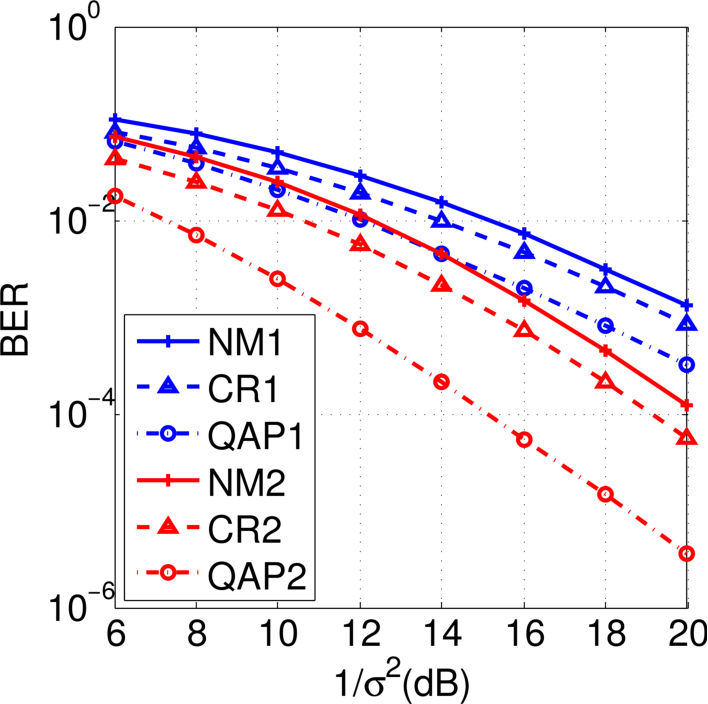
\includegraphics[width=0.9\textwidth]{figs/BER_noise_power_MonteCarlo_64QAM_23.pdf}
      \caption{$m=1,2$.}
    \end{figure}
    
    \column{.5\textwidth}
    \begin{figure}
      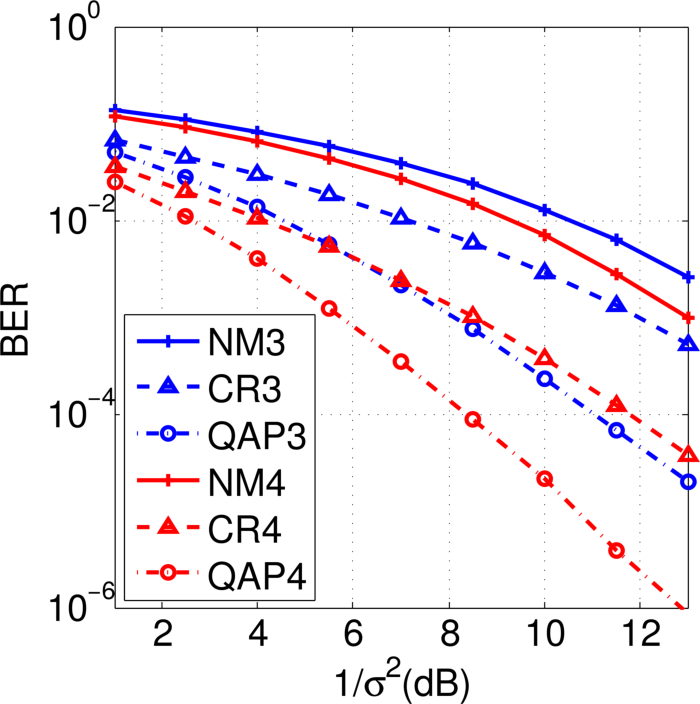
\includegraphics[width=0.9\textwidth]{figs/BER_noise_power_MonteCarlo_64QAM_45.pdf}
      \caption{$m=3,4$.}
    \end{figure}
  \end{columns}
\end{frame}

\begin{frame}
  \frametitle{Numerical Results: Coded BER}
  Add a Forward Error Correction (FEC) code so that
  the coded BER drop rapidly as the noise power is below a certain level. The
  result is termed ``waterfall curve'' which is commonly used to highlight the
  performance gain in dB.
  \begin{columns}
    \column{.5\textwidth}
    \begin{figure}
      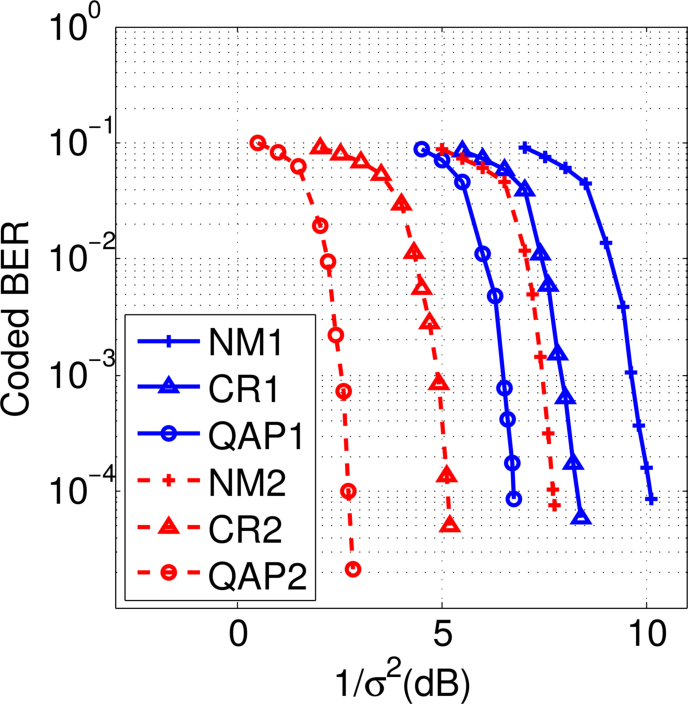
\includegraphics[width=0.9\textwidth]{figs/waterfall_2M3M_64QAM.pdf}
      \caption{$m=1,2$.}
    \end{figure}
    
    \column{.5\textwidth}
    \begin{figure}
      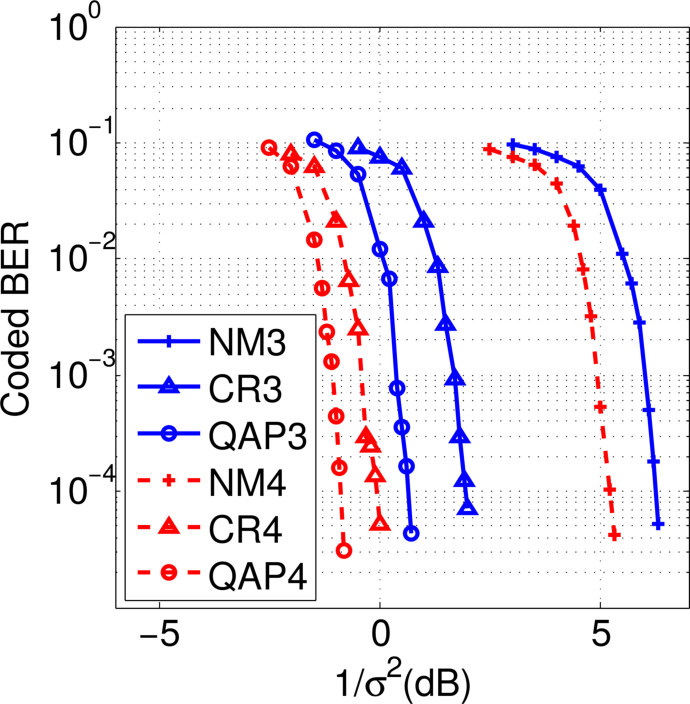
\includegraphics[width=0.9\textwidth]{figs/waterfall_4M5M_64QAM.pdf}
      \caption{$m=3,4$.}
    \end{figure}
  \end{columns}
\end{frame}

\begin{frame}
  \frametitle{Numerical Results: Average Throughput}
  \begin{figure}
    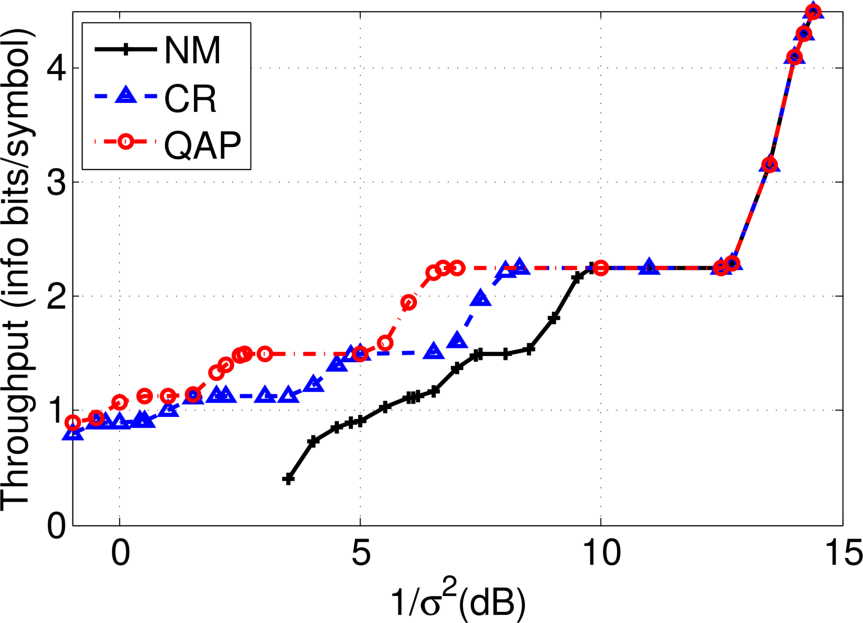
\includegraphics[width=0.7\textwidth]{figs/throughput_6M_64QAM.pdf}
    \caption{Throughput comparison.}
  \end{figure}
\end{frame}

\subsection[MoDiv for MIMO-HARQ]{MoDiv Design for Multiple-Input and
Multiple-Output HARQ Channel}
\begin{frame}
  \frametitle{Multiple-Input and Multiple-Output (MIMO) Channel}
  \begin{figure}
    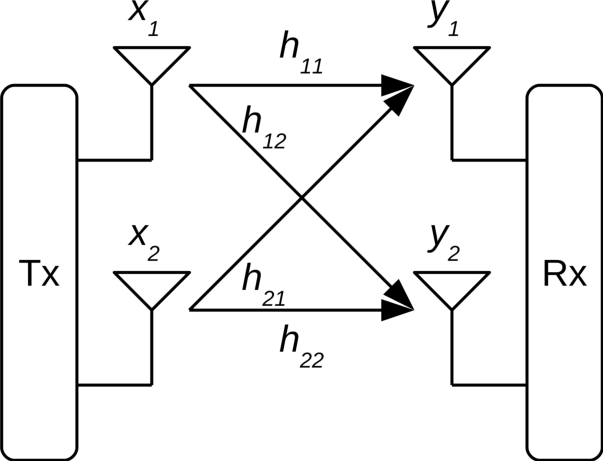
\includegraphics[width=0.5\textwidth]{figs/mimo.pdf}
    \caption{A $2\times 2$ MIMO channel, $y_1 = h_{11}x_1 + h_{21}x_2 + n_1$,
    $y_2 = h_{12}x_1 + h_{22}x_2 + n_2$, or simply $\mathbf{y} = \mathbf{Hx}
    + \mathbf{n}$.}
  \end{figure}
  \begin{itemize}
    \item An essential element in most modern wireless communication standards:
    Wi-Fi, HSPA+, LTE, WiMAX, etc.
    \item How do we generalize the idea of MoDiv design for MIMO channel?
  \end{itemize}
\end{frame}

\begin{frame}[t]
  \frametitle{An Example of CoRe for MIMO}
  \begin{itemize}
    \item<1-> A $1\times 2$ MIMO channel: $\mathbf{H} = [1, 1]$ (simple
    addition).
    \item<1-> Different mapping across the 2 transmitting antennas:
    \item<2-> Effective constellation seen by the receiver: $\psi_e =
    (\bm{\psi})_1 + (\bm{\psi})_2$.
  \end{itemize}
  \begin{columns}
    \column{.5\textwidth}
    \begin{center}
      \includegraphics<1>[width=3cm]{figs/16QAM_Gray_iq.pdf}
      \includegraphics<2>[width=3.5cm]{figs/16QAM_Gray_combined.pdf}
      
      \only<1>{Original transmission (Gray).}
      \only<2>{Effective constellation mapping of the original transmission.}
    \end{center}
    
    \column{.5\textwidth}
    \begin{center}
      \includegraphics<1>[width=3cm]{figs/16QAM_Gray_iq_1.pdf}
      \includegraphics<2>[width=3.5cm]{figs/16QAM_Gray_combined_1.pdf}
      
      \only<1>{1st retransmission.}
      \only<2>{Effective constellation mapping of the 1st retransmission.}
    \end{center}
  \end{columns}
  \vfill
  \only<2>{For HARQ-CC, this CoRe scheme of the 1st retransmission outperforms
  the repeated use of the same Gray mapping across the 2 antennas!}
\end{frame}

\begin{frame}
  \frametitle{MoDiv Design for MIMO Channel}
  \begin{itemize}
    \item MIMO channel model: correlated Rician fading channel
    \begin{align*}
      \mathbf{H}^{(m)} = \sqrt{\frac{K}{K + 1}}
      \underbrace{\mathbf{H}_0}_\text{``Mean''} +
      \sqrt{\frac{1}{K +
      1}}\mathbf{R}^{1/2} \underbrace{\mathbf{H}_w^{(m)}}_\text{``Variation''}
      \mathbf{T}^{1/2}
    \end{align*}
    $K$: Rician factor, $\mathbf{R}, \mathbf{T}$: correlation matrix or the
    receiver and transmitter antennas.
    \item HARQ protocol: HARQ-CC
    \item Design Criterion: BER upperbound based on PEP, successive
    optimization.
  \end{itemize}
  For now we consider the case of $N_T = 2$ (2 transmitting antennas).
\end{frame}

\begin{frame}
  \frametitle{Representation of CoRe}
  Representing the 2-D vector mapping function $\bm{\psi}_m[\cdot]$
  with $Q^3$ binary variables:
  \begin{align*}
    x_{pij}^{(m)} = \left\{ \begin{array}{cc}1 & \mbox{if } \bm{\psi}_m[p] =
    (\psi_0[i], \psi_0[j])^T\\ 0 & \mbox{otherwise.}\end{array} \right. \,
    p, i, j = 0,\ldots, Q - 1
  \end{align*}
  $\psi_0$ represents Gray-mapping for the original transmission (fixed).
  \begin{block}{Constraints: $\bm{\psi}_m[\cdot]$ as a permutation of $0,\ldots,
  Q - 1$}
    \begin{columns}
      \column{.3\textwidth}
      \begin{align*}
        \sum_{i=0}^{Q-1}\sum_{j=0}^{Q-1}x_{pij} & = 1\\
        \sum_{p=0}^{Q-1}\sum_{j=0}^{Q-1}x_{pij} & = 1\\
        \sum_{p=0}^{Q-1}\sum_{i=0}^{Q-1}x_{pij} & = 1
      \end{align*}
      
      \column{.7\textwidth}
      \begin{center}
        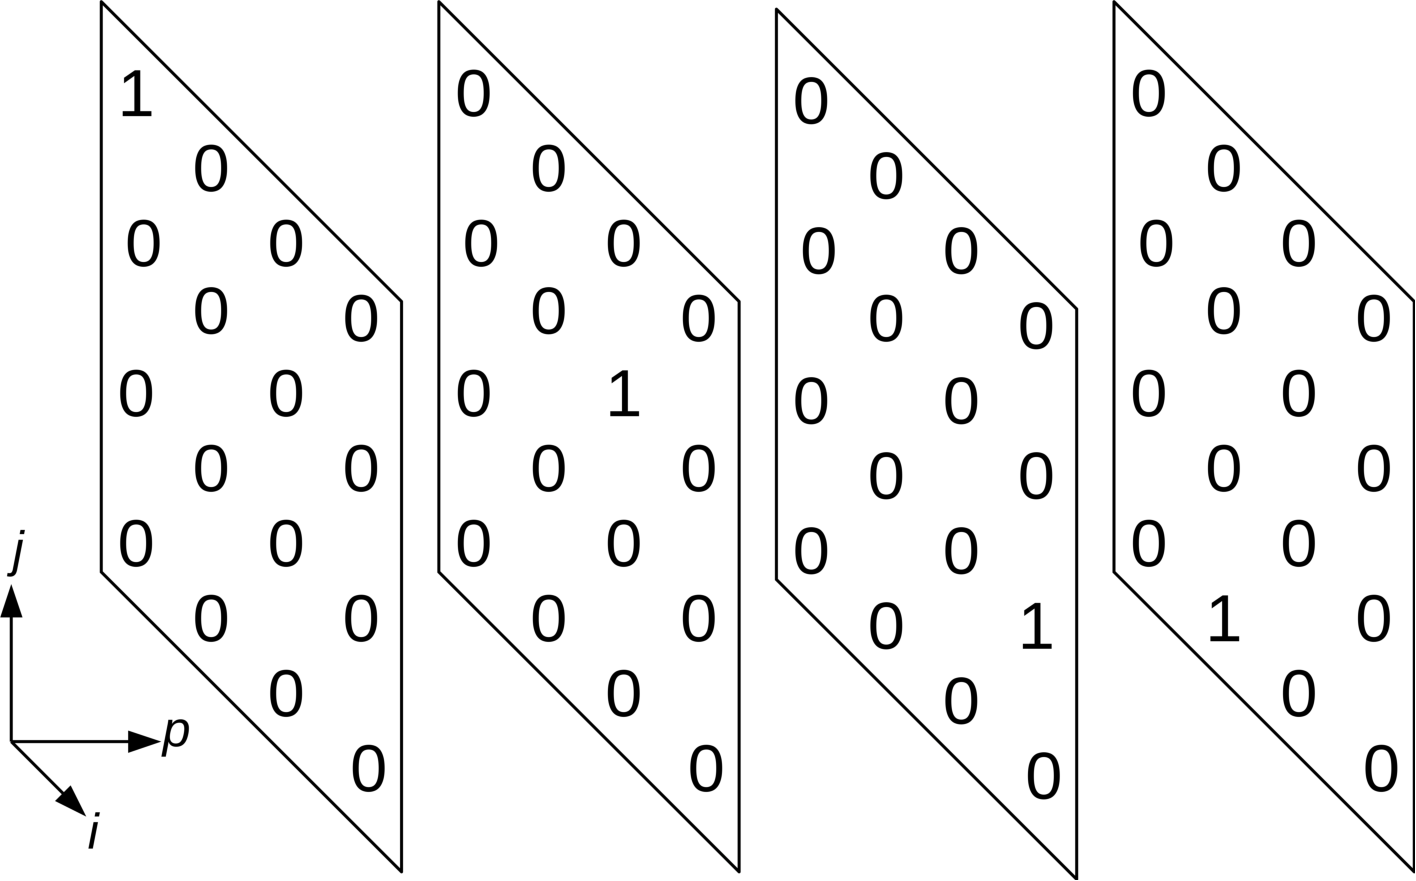
\includegraphics[width=0.7\textwidth]{figs/constraint_q3ap.pdf}
      \end{center}
      
    \end{columns}
  \end{block}
\end{frame}

\begin{frame}
  \frametitle{A Successive Q3AP Formulation}
  \begin{block}{MoDiv design via successive Q3AP}
    \begin{enumerate}[<+->]
      \item Set $m = 1$. Initialize the ``distance'' matrix and the approximated
      PEP, for $p, q, i, j, k, l=0,\ldots,Q-1$:
      \begin{align*}
        d_{ikjl} = \tilde{E}_k[i,j],\; \tilde{P}_{PEP}^{(0)}(q|p) = d_{pqpq}/2
      \end{align*}
      \item Evaluate the ``flow'' matrix:
      \begin{align*}
        f_{pq}^{(m)} = \frac{D[p,q]}{Q\log_2Q}\tilde{P}_{PEP}^{(m-1)}(q|p)
      \end{align*}
      \item Solve the $m$-th Q3AP problem:
      \begin{align*}
        \min_{\{x_{pij}^{(m)}\}}
        \sum_{p=0}^{Q-1}\sum_{i=0}^{Q-1}\sum_{j=0}^{Q-1}
        \sum_{q=0}^{Q-1}\sum_{k=0}^{Q-1}\sum_{l=0}^{Q-1}
        f_{pq}^{(m)}d_{ikjl}x_{pij}^{(m)}x_{qkl}^{(m)}
      \end{align*}
    \end{enumerate}
  \end{block}
\end{frame}

\begin{frame}
  \frametitle{A Successive Q3AP Formulation (Continued)}
  \begin{block}{MoDiv design via successive Q3AP}
    \begin{enumerate}[<+->]
      \setcounter{enumi}{3}
      \item Update PEP:
      \begin{align*}
        \tilde{P}_{PEP}^{(m)}(q|p) & = \sum_{i=0}^{Q-1} \sum_{k=0}^{Q-1}
        \sum_{j=0}^{Q-1} \sum_{l=0}^{Q-1}\tilde{P}_{PEP}^{(m
        - 1)}(q|p)d_{ikjl}\hat{x}_{pij}^{(m)}\hat{x}_{qkl}^{(m)}
      \end{align*}
      where $\hat{x}_{pij}^{(m)}$ is the solution from Step 3.
      \item Increase $m$ by 1, return to Step 2 if $m \leq M$.
    \end{enumerate}
  \end{block}
  \vfill
\end{frame}

\begin{frame}
  \frametitle{Comments}
  
  \begin{itemize}
    \item The $Q^4$ ``distance'' matrix has $Q^4$ elelments. However, for
    $Q$-QAM constellation, it only has $\mathcal{O}(Q^2)$ unique value, can be
    computed more efficiently.
    \item When $N_T > 2$, the MoDiv design can be formulated into a quadratic
    $(N_T + 1)$-dimensional problem, with $Q$-by-$Q$ ``flow'' matrix and $Q ^
    {2N_T}$ ``distance'' matrix, which might be too complex to solve. However,
    one can always apply a $N_T$-by-$2$ linear precoding matrix to reduce the
    channel into a $N_R$-by-$2$ channel to partly explore modulation diveristy.
  \end{itemize}
\end{frame}


\begin{frame}
  \frametitle{Numerical Results: Simulation Settings}
  \begin{itemize}[<+->]
    \item 64-QAM constellation ($Q = 64$).
    \item Maximum number of 4 retransmissions ($M = 4$).
    \item Correlated Rician-fading channels, $\mathbf{H}_0 = [1, 1]$,
    correlation factor $\rho = 0.7$.
    \item Use a modified iterative local search algorithm\footnotemark to
    solve each Q3AP numerically.
    \item Compare 3 MoDiv schemes:
      \begin{enumerate}
        \item No modulation diversity with maximum SNR beam-forming (NM).
        \item A heuristic CoRe scheme for HSPA with maximum SNR
        beam-forming (CR).
        \item Q3AP-based solution (Q3AP).
      \end{enumerate}
  \end{itemize}
  \footnotetext[1]{T. St\"{u}tzle, and D. Marco, ``Local search and
  metaheuristics for the quadratic assignment problem,'' Technical Report
  AIDA-01-01, Intellectics Group, Darmstadt University of Technology, Germany,
  2001.}
\end{frame}

\begin{frame}
  \frametitle{Numerical Results: Uncoded BER vs Noise Power}
  \begin{columns}
    \column{.5\textwidth}
    \begin{figure}
      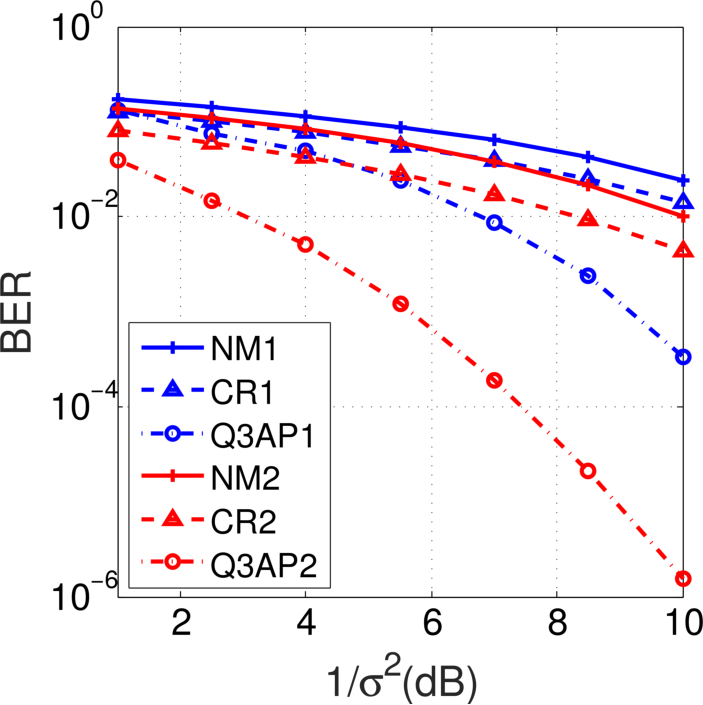
\includegraphics[width=0.9\textwidth]{figs/BER_noise_power_MonteCarlo_64QAM_23_Q3AP.pdf}
      \caption{$m=1,2$.}
    \end{figure}
    
    \column{.5\textwidth}
    \begin{figure}
      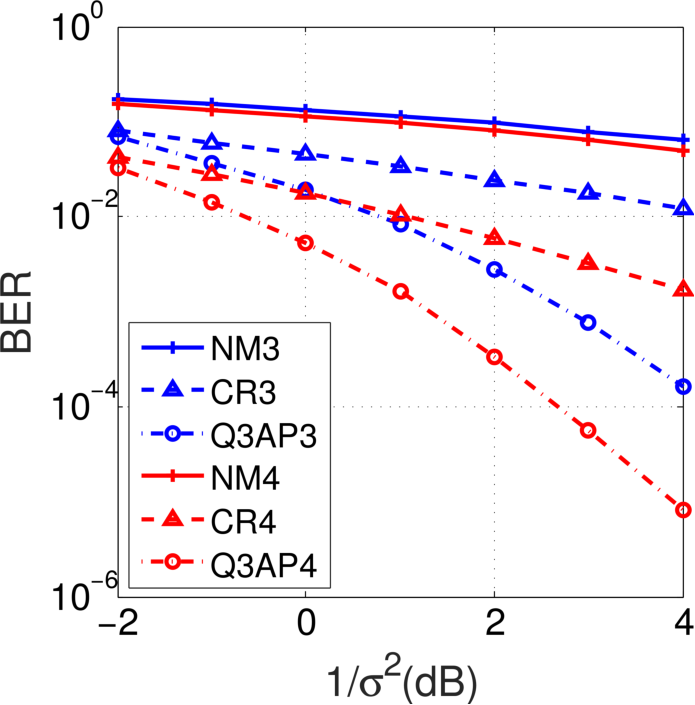
\includegraphics[width=0.9\textwidth]{figs/BER_noise_power_MonteCarlo_64QAM_45_Q3AP.pdf}
      \caption{$m=3,4$.}
    \end{figure}
  \end{columns}
\end{frame}

\begin{frame}
  \frametitle{Numerical Results: Uncoded BER vs $K$}
  Larger $K$ $\leftrightarrow$ the channel is less random.
  \begin{columns}
    \column{.5\textwidth}
    \begin{figure}
      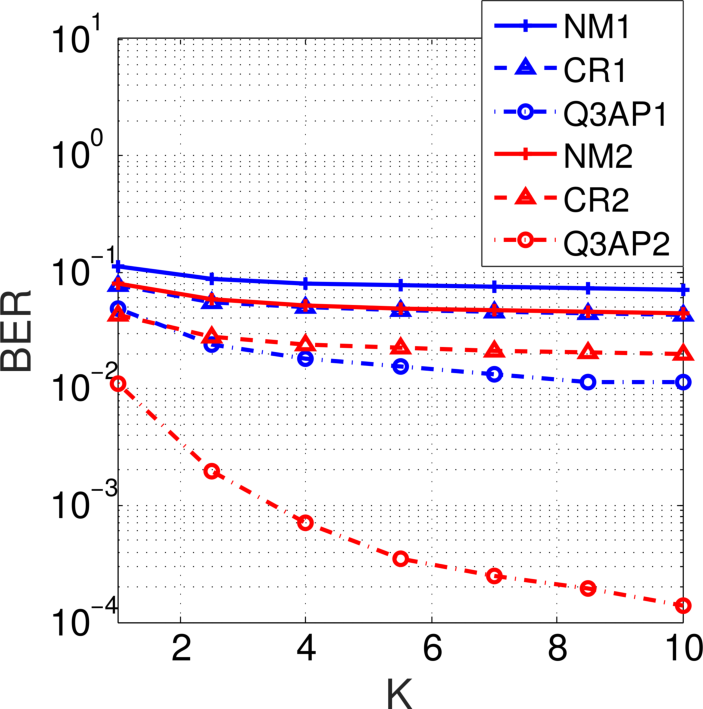
\includegraphics[width=0.9\textwidth]{figs/BER_K_MonteCarlo_64QAM_6.pdf}
      \caption{$m=1,2$, $1/\sigma^2 = 6dB$.}
    \end{figure}
    
    \column{.5\textwidth}
    \begin{figure}
      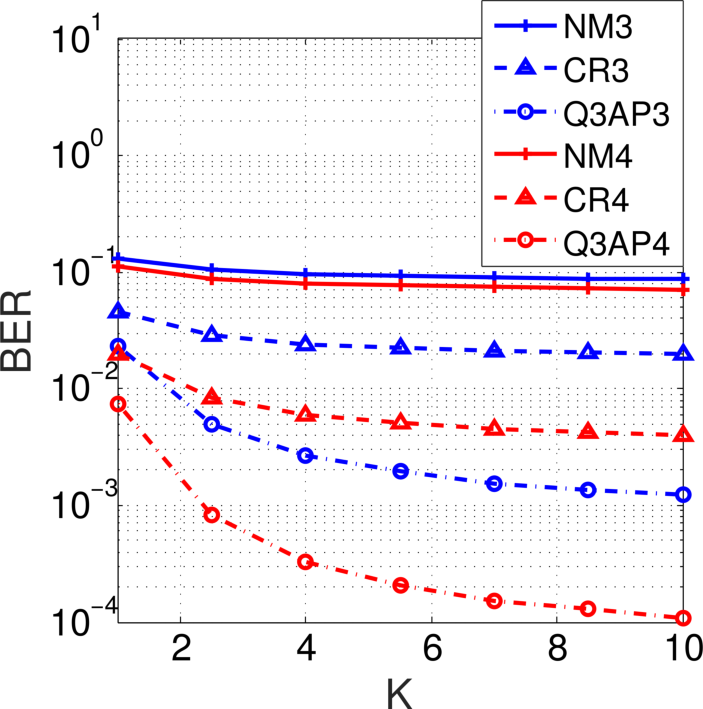
\includegraphics[width=0.9\textwidth]{figs/BER_K_MonteCarlo_64QAM_2.pdf}
      \caption{$m=3,4$, $1/\sigma^2 = 2dB$.}
    \end{figure}
  \end{columns}
\end{frame}

\begin{frame}
  \frametitle{Numerical Results: Coded BER}
  \begin{columns}
    \column{.5\textwidth}
    \begin{figure}
      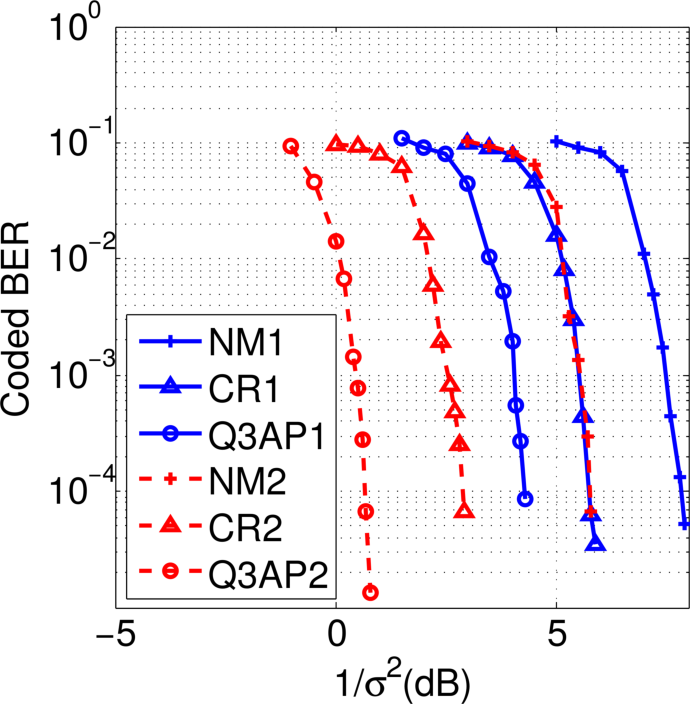
\includegraphics[width=0.9\textwidth]{figs/waterfall_2M3M_64QAM_Q3AP.pdf}
      \caption{$m=1,2$.}
    \end{figure}
    
    \column{.5\textwidth}
    \begin{figure}
      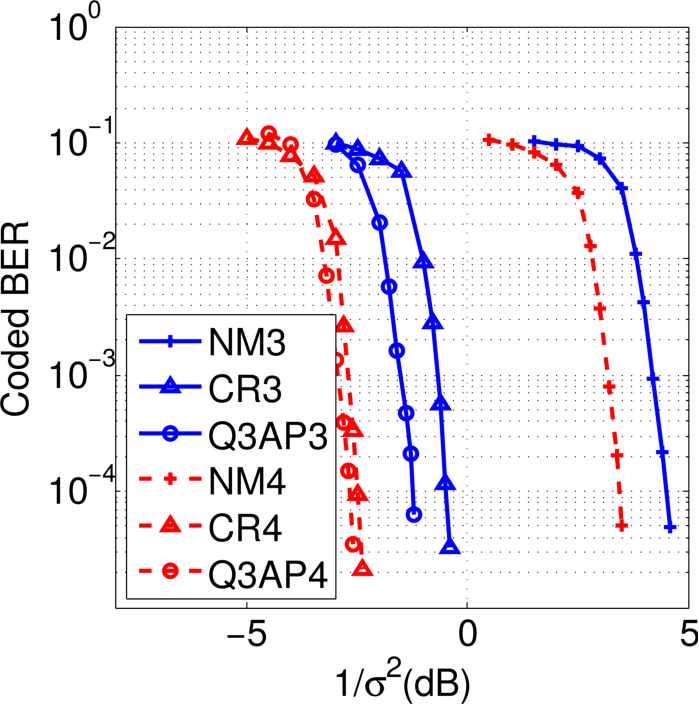
\includegraphics[width=0.9\textwidth]{figs/waterfall_4M5M_64QAM_Q3AP.pdf}
      \caption{$m=3,4$.}
    \end{figure}
  \end{columns}
\end{frame}

\begin{frame}
  \frametitle{Numerical Results: Average Throughput}
  \begin{figure}
    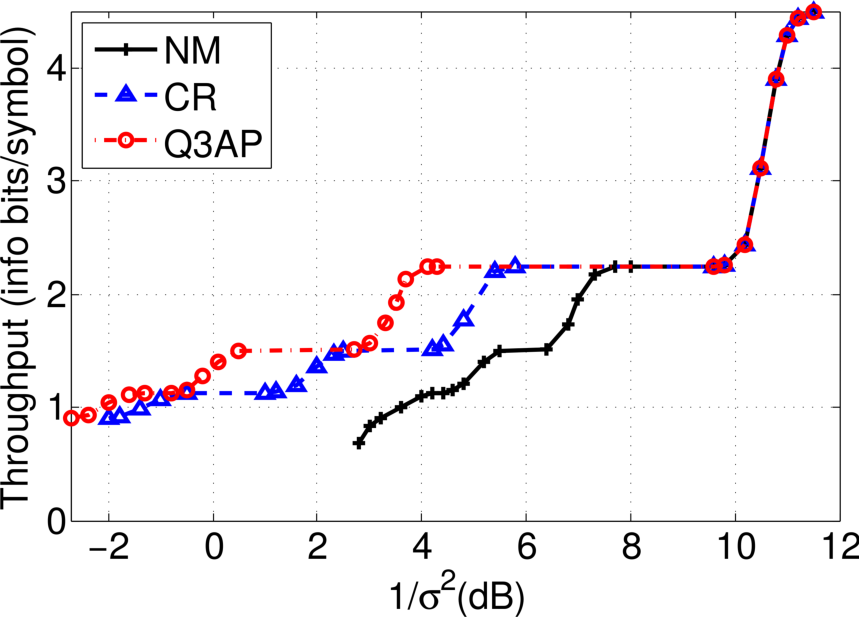
\includegraphics[width=0.7\textwidth]{figs/throughput_5M_64QAM_Q3AP.pdf}
    \caption{Throughput comparison.}
  \end{figure}
\end{frame}

\subsection{Conclusion}
\begin{frame}
  \frametitle{Conclusion}
  \begin{itemize}[<+->]
    \item Formulate Modulation Diversity (MoDiv) design for wireless
    communication system into Quadratic Assignment Problems (QAPs):
    \begin{enumerate}
      \item Two-Way Relay Analog Network Coding Rayleigh-fading channel:
      successive Koopman-Beckmann QAP.
      \item Correlated Rician-fading Multiple-Input and Multiple-Output channel:
      successive Q3AP.
    \end{enumerate}
    \item Significant performance gain for a wide range of settings over
    existing heuristic MoDiv schemes. 
  \end{itemize}
\end{frame}
%------------------------------------------------

%----------------------------------------------------------------------------------------

\end{document}